\documentclass[UTF8]{ctexart}
\usepackage[a4paper,left=3cm,right=3cm,top=2cm]{geometry}
\usepackage{amsmath}
\usepackage{enumitem}
\usepackage{float}
\usepackage{threeparttable}
\usepackage{caption}
\usepackage{multirow}
\usepackage{graphicx}
\usepackage{listings}
\usepackage{xcolor}
\usepackage{amssymb}
\usepackage[colorlinks,linkcolor=blue]{hyperref}
\renewcommand{\figurename}{Figure}
\definecolor{dkgreen}{rgb}{0,0.6,0}
\definecolor{gray}{rgb}{0.5,0.5,0.5}
\definecolor{mauve}{rgb}{0.58,0,0.82}
\lstdefinelanguage{LC3}{
  morekeywords={ADD, AND, BR, BRn, BRnz, BRnzp, BRnp, BRz, BRzp, BRp, JMP, JSR, LD, LDI, LDR, LEA, NOT, ST, STI, STR},
  sensitive=false,
  morecomment=[l]{;},
  morestring=[b]",
  morekeywords=[2]{R0, R1, R2, R3, R4, R5, R6, R7}, % Define register keywords
}
\lstset{frame=tb,
  language=LC3,
  aboveskip=3mm,
  belowskip=3mm,
  showstringspaces=false,
  columns=flexible,
  basicstyle={\small\ttfamily},
  numbers=left,%设置行号位置none不显示行号
  numberstyle=\tiny\courier, %设置行号大小
  numberstyle=\tiny\color{gray},
  keywordstyle=\color{blue},
  keywordstyle=[2]\color{purple},
  commentstyle=\color{dkgreen},
  stringstyle=\color{mauve},
  breaklines=true,
  breakatwhitespace=true,
  escapeinside=`,%逃逸字符(1左面的键),用于显示中文例如在代码中`中文...`
  tabsize=4,
  extendedchars=false %解决代码跨页时,章节标题,页眉等汉字不显示的问题
}

\setlength\lineskiplimit{5.25bp}
\setlength\lineskip{5.25bp}

\title{Lab5 Report}
\author{崔士强 PB22151743}
\date{December 24, 2023}

\begin{document}

\maketitle
\section{Program Design}
The structure of the program is shown in the following figure. 
The function TERM stands for TERMination.
\begin{figure}[H]
  \centering
  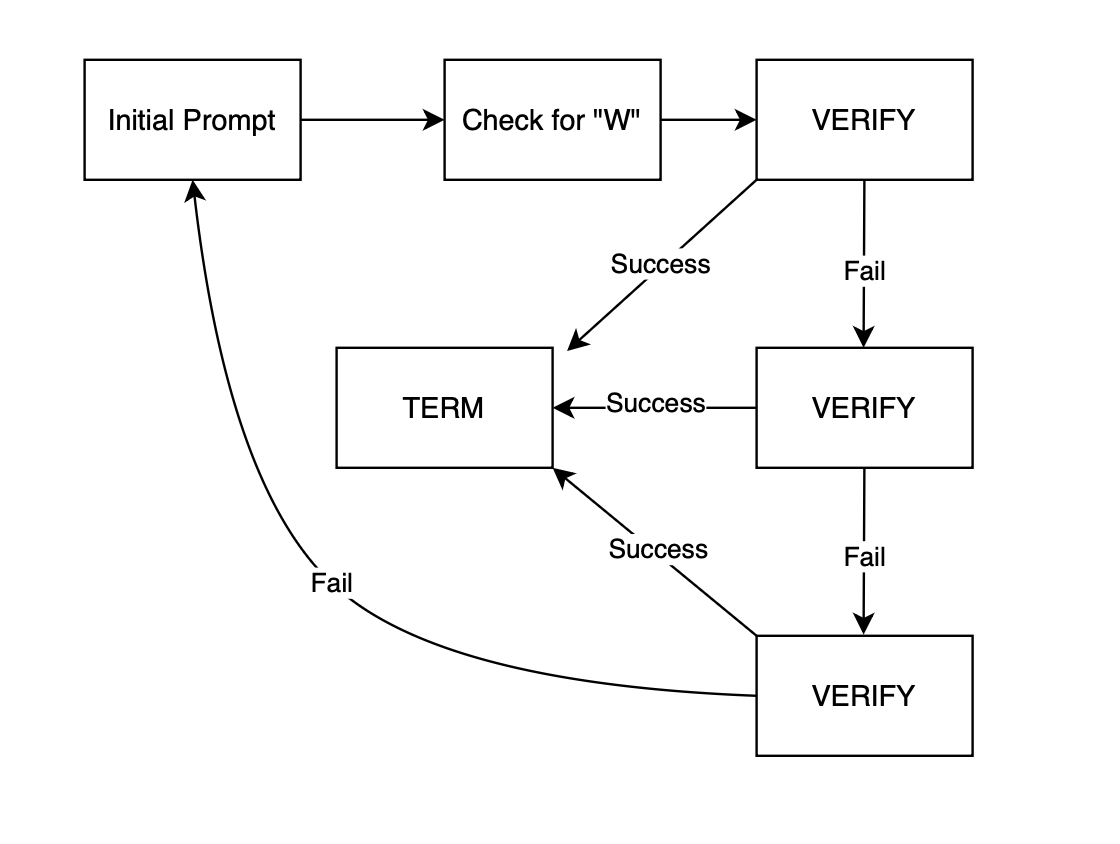
\includegraphics[scale=0.5]{Overall.png}
  \caption{Overall structure}
\end{figure}

Here is the details of the function VERIFY. It reads a character each time and
compare it to the corresponding character in the password. 
If an unmatching character is found or the length of input
exceeds the password. The indicator(i.e. \lstinline{R0}) is set negative.
\begin{figure}[H]
  \centering
  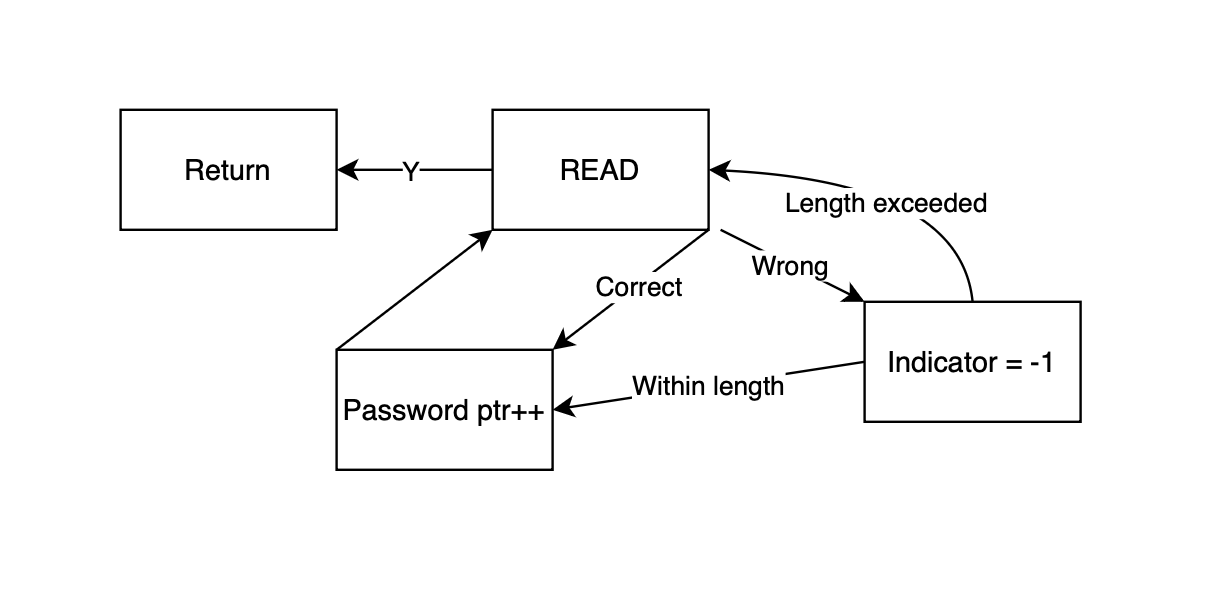
\includegraphics[scale=0.5]{Verify.png}
  \caption{Details of VERIFY}
\end{figure}

\section{Testing Evidence}
Screen recording: \href{https://rec.ustc.edu.cn/share/ed2c2e60-a262-11ee-861b-01b0339fadfa}{Program test} 
\section{Discussion Questions}
\subsection{Functions}
Several functions are used in the program. Reasons:
\begin{enumerate}
  \item Some part of the program may be executed more than once.
  \item The use of functions increases readability and makes debugging easier.
\end{enumerate}
\subsection{Recursion}
Recursive functions can be used in the program for checking password. But due to the simplicity of the process
(10-character password and 3 attempts), I chose not to use them. 

Also, the use of recursion to check password may have a problem when input is 
super long.

Actually attempts and preparations to use recursion was made.
\subsection{Preset Prompts}
In this program, only 3 attempts are allowed, which means prompts are not too many. 
In order to keep developing process simple, all prompts are stored using \lstinline{.STRINGZ}
, rather than combine prompts for incorrect inputs, which is a resonable approach if number of attempts allowed may be modified.
\begin{lstlisting}
  INITPRPT      .STRINGZ    "Welcome to the bank system! Type 'W' to withdraw some fund."
  SUCCPRPT      .STRINGZ    "Success!"
  FAILIPRPT     .STRINGZ    "Incorrect password! 2 attempts remaining."
  FAILIIPRPT    .STRINGZ    "Incorrect password! 1 attempt remaining."
  FAILIIIPRPT   .STRINGZ    "Fails."
  INPUTPRPT     .STRINGZ    "Please input your password:"
  PSWD          .STRINGZ    "PB22151743"
\end{lstlisting}
\subsection{Program Security}
There are two kinds of inputs worth considering: empty input and long input.

In this program, the length of input won't cause a problem. 
Every time a character is read by the program, it's immediately
checked. If the input is longer than the password or a wrong character is found, 
the indicator will be kept negative. 

As for the empty input, A register is set to mark the first character. 
If the first character is Y, the indicator will be nagative.

\subsection{Challenges}

An error occured when I tried to assemble the program, which I had
never met before:
\begin{figure}[H]
    \centering
    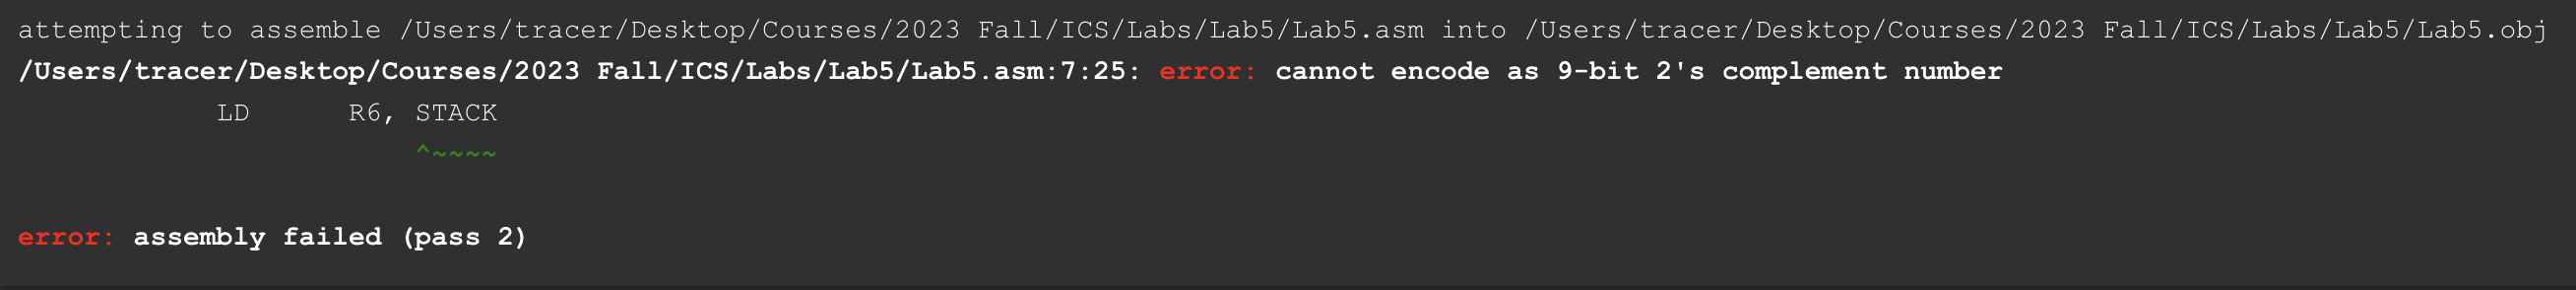
\includegraphics[scale=0.3]{Error1.png}
    \caption{An error}
\end{figure}

The same instruction worked well in Lab4, which baffled me. Later I realized what 
the message means: PCoffset was too large. 

Solution: move the instruction up.

\end{document}
\iffalse
\begin{figure}[H]
    \centering
    \includegraphics[scale=0.5]{name.png}
    \caption{name}
\end{figure}
\fi
